\documentclass[12pt,a4paper]{report}
\usepackage{amsmath}
\usepackage{amssymb}
\usepackage{mathabx}
\usepackage{stmaryrd}
\usepackage{upgreek}
\usepackage{graphicx}
\usepackage{fancyhdr}
\usepackage{enumerate}
\usepackage[vmargin=2.5cm, hmargin=2.5cm]{geometry}
\usepackage{hyperref}
\usepackage{fontspec}
\usepackage{unicode-math}
\usepackage{stackengine}
\usepackage{minitoc}
\usepackage{amsthm}
\usepackage{listings}
\usepackage{xcolor}
\usepackage{xeCJK}
\usepackage{dirtree}
\usepackage{float}
\usepackage{pdfpages}
\usepackage{atbegshi}
\usepackage{multirow, makecell}
\usepackage{enumitem}
\usepackage{hhline}


\setmainfont{Linux Libertine O}
\setsansfont{Linux Biolinum O}
\setCJKmainfont{Noto Serif CJK JP}

\graphicspath{{./fig/category_theory/}{./fig/agda/lagda/latex/}{./fig/implementation/}{./proposal/}{./code/}}

\setlength{\parindent}{0em}
\addtolength{\parskip}{1ex}

\usepackage[backend=biber,bibstyle=ieee,citestyle=numeric-comp]{biblatex}
\addbibresource{ref.bib}

\theoremstyle{definition}
\newtheorem{definition}{Definition}[chapter]

\newtheorem{theorem}[definition]{Theorem}

\newtheorem{example}[definition]{Example}

\newtheorem{prf}[definition]{Proof Sketch}

\newcounter{motivation}
\renewcommand{\themotivation}{\Roman{motivation}}

\newcommand{\motivation}[1]{%
    \refstepcounter{motivation}%
    \vspace{1.5em}%
    \noindent\textbf{Motivation \themotivation.  #1}
    \par
    \expandafter\edef\csname savedmotivation\themotivation\endcsname{%
        \noexpand\noindent\noexpand\textbf{Motivation \themotivation. #1}\noexpand\par
    }%
}

\newcommand{\secref}[1]{\S\ref{#1}}
\newcommand{\chapref}[1]{\ref{#1}}

\definecolor{mediumblue}{HTML}{0000CD}
\definecolor{green}{HTML}{008B00}
\definecolor{orange}{HTML}{CD6600}
\definecolor{darkpink}{HTML}{EE1289}

\newcommand{\mb}[1]{\textcolor{mediumblue}{#1}}
\newcommand{\gn}[1]{\textcolor{green}{#1}}
\newcommand{\og}[1]{\textcolor{orange}{#1}}
\newcommand{\dpink}[1]{\textcolor{darkpink}{#1}}

\newcommand{\bN}{\mathbb{N}}
\newcommand{\bZ}{\mathbb{Z}}

\newcommand{\yo}{\mathord{\text{\kern0.03em \scalebox{0.8}{よ}\kern0.03em}}}

\newcommand{\bracket}[1]{\left\{ #1 \right\}}
\newcommand{\ang}[1]{\left\langle #1 \right\rangle}
\newcommand{\intp}[1]{\left\llbracket #1 \right\rrbracket}

\newcommand{\frontmatter}{
  \pagenumbering{roman}
}

\newcommand{\mainmatter}{
  \cleardoublepage
  \pagenumbering{arabic}
  \setcounter{page}{1}
}

\renewcommand{\arraystretch}{1.5}

\begin{document}

\dominitoc

\begin{titlepage}
    \begin{flushright}
        \textbf{\Large Jack Gao}
    \end{flushright}
    
    \vspace{12em}

    \begin{center}
        \textbf{\huge Using functor categories to generate intermediate code with Agda}
        \vspace{3em}

        {\Large Computer Science Tripos - Part II Dissertation}
        \vspace{1em}

        {\Large Homerton College}
        \vspace{1em}

        {\large \today}
    \end{center}
\end{titlepage}

\begin{titlepage}
    \vspace*{5em}
    \textbf{\LARGE Declaration of Originality}
    \vspace{2em}

    I, the candidate for Part II of the Computer Science Tripos with Blind Grading Number 2330G, hereby declare that this report and the work described in it are my own work, unaided except as may be specified below, and that the report does not contain material that has already been used to any substantial extent for a comparable purpose. In preparation of this report, I adhered to the Department of Computer Science and Technology AI Policy. I am content for my report to be made available to the students and staff of the University.
    \vspace{1em}

    Date: \today
\end{titlepage}

\begin{titlepage}
    \vspace*{5em}
    \textbf{\LARGE Proforma}
    \vspace{2em}

    \begin{tabular}{ll}
        \textbf{Candidate Number:} & 2330G \\
        \textbf{Title of Project:} & Using functor categories to generate intermediate code with Agda \\
        \textbf{Examination} & Computer Science Tripos - Part II - 2025 \\
        \textbf{Word-count:} & [wordcount] \footnotemark \\
        \textbf{Code line count:} & [linecount] \footnotemark \\
        \textbf{Project Originator:} & Yulong Huang \\
        \textbf{Project Supervisor:} & Yulong Huang and Yufeng Li \\
    \end{tabular}

    \vspace{2em}
    \textbf{\Large Original Aims of the Project}
    \vspace{1em}

    \vspace{2em}
    \textbf{\Large Work Completed}
    \vspace{1em}

    \vspace{2em}
    \textbf{\Large Special Difficulties}
    \vspace{1em}
    \begingroup
        \footnotetext[1]{This word-count was computed by \texttt{texcount -1 -sum -merge -q dissertation.tex}.}
        \footnotetext[2]{This code line count was computed by \texttt{find . -name "*.agda" | xargs wc -l}.}
    \endgroup
\end{titlepage}

\frontmatter
\tableofcontents
\newpage

\mainmatter
\chapter{Introduction}
    \minitoc
    Programming languages act as a bridge between human thoughts and machine execution. They exist in two complementary realms: the human realm, where intent is expressed through abstractions like variables and functions, and the machine realm, where low-level instructions are executed on hardware. 

    Denotational semantics is related to the human realms. It provides a theoretical framework for defining the meaning of programming languages by interpreting them into mathematical objects. By formalising the denotational semantics of a programming language, we ensure that its abstraction align with our intentions.

    Compilers are related to the machine realms. They are programs that translate high-level code into executable instructions, resolving abstractions into concrete operations like memory allocation and register management. Compilers are essential for turning human-written code into physical computation.

    This project explores how the two process can be deeply connected by demonstrating how denotational semantics can directly generate a compiler. Simply typed lambda calculus (STLC)~\autocite{stlc} is a well-studied programming language that serves as a foundation for many modern languages. It has denotational semantics in cartesian closed categories (CCC)~\autocite{lambek}. As a CCC, presheaf categories over store locations can be used to model STLC with stores, as shown by by Reynolds~\autocite{essence} and Oles~\autocite{Oles_1,Oles_2}. Later, Reynolds presented a denotational semantics of STLC with stores in the form of a presheaf category over compiler states~\autocite{Reynolds}. By interpreting the source language into the presheaf category over \emph{stack descriptors}, where objects of the category represent instruction sequences parametrised by stack layouts, the semantic model directly yields a compiler. 
    
    In this dissertation, I implement Reynolds' presheaf-based compiler for STLC with stores in a dependently typed programming language, Agda~\autocite{Agda}. The compiler is a \emph{functor} (structure-preserving map) from the source language to the target language. The implementation is verified with Agda, which ensures that the input source program, the compilation process, and the output target program are all well-typed.

    This work both validates and refines Reynolds' theory, offering a concrete example of how category-theoretic semantics can generate intermediate code. The project also serves as a practical demonstration of the power of dependently typed programming languages can mechanise the link between theory and practice.

    \section{Motivation} \label{sec: motivation}
        This project is motivated and guided by the following:
        
        \motivation{Formal verification of the compiler}
        Reynolds' work presented detailed definitions of denotational semantics of STLC with stores, which are complicated and error-prone. The rise of verified compilers including CompCert~\autocite{CompCert} and CakeML~\autocite{CakeML} reflects a broader trend toward trustworthy systems, where correctness proofs replace testing for critical guarantees. I aim to provide a formalisation of the definition in a proof assistant to verify the correctness of the given denotational semantics.

        \motivation{Implementation of the compiler}
        Reynolds concluded that he did not have a proper dependently typed programming language in hand, so his compiler remained a partial function~\autocite[Ch.6]{Reynolds}. I aim to provide a computer implementation of this theoretical framework in a dependently typed programming language.

    
    \section{Language choice: Agda's advantages}
        Agda~\autocite{Agda} is a dependently typed programming language and proof assistant. Agda captures the source language's intrinsic syntax with indexed families, which contains only well-typed terms. Therefore, it focuses on the correct programs and rules out the ill-typed nonsensical inputs. 

        Dependently typed languages provide a natural framework for expressing functor categories is proven both theoretically and practically. There have been dependent-type-theoretic model of categories~\autocite{Dybjer}, and it has been shown that functor categories arise naturally as dependent function types~\autocite{Jacobs}. A formalisation of Category Theory, including cartesian closed categories, functors and presheaves has been developed in Agda by Hu and Caratte~\autocite{Cat_Agda}. Other proof assistants, such as Isabelle/Hol, does not have a dependently typed language structure, and thus cannot express the functor categories as naturally as Agda. 

        Compared to other dependently typed languages, Agda is more balanced in terms of programming and proving. Its \og{\textsf{with}}-abstraction and \og{\textsf{rewrite}} construction allow for a more flexible and powerful way to define and manipulate terms. The \og{\textsf{with}}-abstraction allows us to inspect intermediate values in a term, which gives a refined view of a function's argument. The \og{\textsf{rewrite}} construction allows us to define new terms by expanding existing terms, which avoids rewriting proofs of similar structures.

        Agda also provides an interactive environment for writing and verifying programs, which will be further discussed in~\secref{subsec: holes}.

    \section{Contributions}
        Addressed the two motivations presented in~\secref{sec: motivation} and contributed to the following:
        \begin{quote}            
            \savedmotivationI
            I formalised the terms in the source language and target language in Agda. I also refined some type definitions in the denotational semantics of the source language.
            
            \savedmotivationII
            I implemented the compiler from the source language to the target language in Agda. 
        \end{quote}


\chapter{Preparation}
    \minitoc

    For implementing the compiler, I need to understand the theoretical background of presheaves and functor categories that are used as the denotational semantics of the source language, and I need to understand Agda's dependent types to correctly express the dependent function space of presheaf exponentials. This chapter begins with my starting point and an introduction to category theory, followed by a brief overview of the dependently typed programming language Agda, and requirements analysis of the compiler.

    \section{Starting Point}
    Prior to this project, I had no experience with Agda. Although I was aware of the open-source online tutorial \textit{Programming Language Foundations in Agda} (PLFA)~\autocite{plfa}, my preparation was limited to setting up the Agda environment on my laptop by following the ``Front Matter'' section of the tutorial.

    I did not have any other experience with compiler beyond Part IB Compiler Construction Course. I had no prior exposure to category theory and type theory before the Part II lectures.


    \section{Category theory} \label{sec: cat}
        Category theory provides a high-level abstraction from which we can reason about the structure of mathematical objects and their relationships. It provides us a ``bird's eye view'' of the mathematics which enable us to spot patterns that are difficult to see in the details~\autocite{basic_cat}. More specifically, it provides a ``purer'' view of functions that is not derived from sets~\autocite{scott-lambda}. Compared to set theory which is ``element-oriented'', category theory is ``function-oriented'' and ``morphism-oriented''. We understand structures not via elements but by how they transform into each other. 

        Notation in category theory is similar to that in set theory and type theory. For example, $A, B, \dots$ are used to denote objects, sets, or types, and arrows are used to denote morphisms or functions (e.g.\ $A \to B$). There is a deeper connection between category theory and type theory, which will be discussed in~\secref{subsec: curry-howard-lambek}. 

        The following is a brief introduction to the basic concepts of category theory, which is based on the work of Leinster~\autocite{basic_cat}, 
        Riehl~\autocite{cat_context}, and the lecture notes of Part II Category Theory by Andrew Pitts and Marcelo Fiore~\autocite{cat_lecture_notes}.

        \subsection{Category}
        \begin{definition}[Category]
            A \emph{category} $\mathcal{C}$ is specified by
            \begin{itemize}
                \item 
                    a collection of objects $\textbf{obj}(\mathcal{C})$, whose elements are called $\mathcal{C}$-objects;
                \item 
                    for each $X, Y \in \textbf{obj}(\mathcal{C})$, a collection of morphisms $\mathcal{C}{(X,Y)}$, whose elements are called $\mathcal{C}$-morphisms from $X$ to $Y$ (e.g.\ $f : X \to Y$);
                \item 
                    for each $X \in \textbf{obj}(\mathcal{C})$, an element $\textbf{id}_X \in \mathcal{C}{(X,X)}$ called the identity morphism on $X$;
                \item 
                    for each $X, Y, Z \in \textbf{obj}(\mathcal{C})$, a function 
                    \[\begin{aligned}
                        \mathcal{C}{(X,Y)} \times \mathcal{C}{(Y,Z)} &\to \mathcal{C}{(X,Z)} \\
                        (f,g) &\mapsto g \circ f
                    \end{aligned}\]
                    called the composition of morphisms;
            \end{itemize}
            satisfying the following properties:
            \begin{itemize}
                \item 
                    \textbf{(Unit Laws)}
                    For all $X, Y \in \textbf{obj}(\mathcal{C})$ and $f \in \mathcal{C}{(X,Y)}$, we have
                    \begin{equation} \label{law: unit}
                        \textbf{id}_Y \circ f = f = f \circ \textbf{id}_X
                    \end{equation}
                \item
                    \textbf{(Associativity Law)}
                    For all $X, Y, Z, W \in \textbf{obj}(\mathcal{C})$ and $f \in \mathcal{C}{(X,Y)}$, $g \in \mathcal{C}{(Y,Z)}$, $h \in \mathcal{C}{(Z,W)}$, we have
                    \begin{equation} \label{law: associativity}
                        h \circ (g \circ f) = (h \circ g) \circ f
                    \end{equation}
            \end{itemize}
        \end{definition}

        \begin{example}[$\mathcal{Set}$]
            An example of category is the category of sets, denoted as $\mathcal{Set}$, specified by the following:
            \begin{itemize}
                \item 
                    The objects of $\mathcal{Set}$ are a fixed universe of sets;
                \item
                    For each $X, Y \in \textbf{obj}(\mathcal{Set})$, the morphisms from $X \to Y$ in $\mathcal{Set}$ are the functions $X \to Y$;
                \item
                    The identity morphism on $X$ in $\mathcal{Set}$ is the identity function on $X$;
                \item
                    The composition of morphisms in $\mathcal{Set}$ is defined as the composition of functions.
            \end{itemize}
            Associativity law and unit laws are satisfied in $\mathcal{Set}$, since the composition of functions is associative and the identity function compose with any function is the function itself.
        \end{example}

        \begin{definition}[Preorder]
            A \emph{preorder} $\underline{P} = (P, \sqsubseteq)$ is a set $P$ with a binary relation $\sqsubseteq$ that is
            \begin{itemize}
                \item reflexive: $\forall x \in P, x \sqsubseteq x$;
                \item transitive: $\forall x, y, z \in P, x \sqsubseteq y \land y \sqsubseteq z \implies x \sqsubseteq z$.
            \end{itemize}
        \end{definition}

        \begin{example}[Category determined by preorder] \label{ex: category_preorder}
            Another example of category is a category $\mathcal{C}_{\underline{P}}$ determined by any preorder $\underline{P}$, which is specified by the following:
            \begin{itemize}
                \item 
                    The objects of $\mathcal{C}_{\underline{P}}$ are the elements of $P$;
                \item
                    $\mathcal{C}_{\underline{P}}(x,y) = \begin{cases}
                        \{(x,y)\} & \text{if $x \sqsubseteq y$} \\
                        \emptyset & \text{otherwise}
                    \end{cases}$
                \item
                    The identity morphism on $X$ in $\mathcal{C}_{\underline{P}}$ is the identity function on $X$;
                \item
                    The composition of morphisms in $\mathcal{C}_{\underline{P}}$ is defined as the composition of functions.
            \end{itemize}
            Associativity law and unit laws are satisfied in $\mathcal{C}_{\underline{P}}$.

            $\mathcal{C}_{\underline{P}}$ is used later for stack descriptors in the denotational semantics of the source language.
        \end{example}

            \subsubsection{Opposite category}
            The idea of opposite category is that if we have a category $\mathcal{C}$, we can reverse the direction of all morphisms in $\mathcal{C}$ to obtain a new category $\mathcal{C}^{\textbf{op}}$.

            \begin{definition}[Opposite category]
                Given a category $\mathcal{C}$, its \emph{opposite category} $\mathcal{C}^{\textbf{op}}$ is specified by the following:
                \begin{itemize}
                    \item 
                        The objects of $\mathcal{C}^{\textbf{op}}$ are the same as those of $\mathcal{C}$;
                    \item 
                        For each $X, Y \in \textbf{obj}(\mathcal{C})$, the morphisms from $X$ to $Y$ in $\mathcal{C}^{\textbf{op}}$ are the morphisms from $Y$ to $X$ in $\mathcal{C}$;
                    \item 
                        The identity morphism on $X$ in $\mathcal{C}^{\textbf{op}}$ is the identity morphism on $X$ in $\mathcal{C}$;
                    \item 
                        The composition of morphisms in $\mathcal{C}^{\textbf{op}}$ is defined as the composition of morphisms in $\mathcal{C}$.
                \end{itemize}
            \end{definition}

                % \paragraph{The principle of duality}
                % Whenever one defines a concept or proves a theorem in category theory $\mathcal{C}$, one can obtain another concept or theorem in the opposite category $\mathcal{C}^{\textbf{op}}$, called the \emph{dual} of the original concept or theorem, by reversing all arrows in the original concept or theorem.

            The notation of commutative diagram is widely used in category theory as a convenient visual representation of the relationships between objects and morphisms in a category.
            \subsubsection{Commutative diagrams}
            A \emph{diagram} in a category $\mathcal{C}$ is a directed graph whose vertices are $\mathcal{C}$-objects and whose edges are $\mathcal{C}$-morphisms.

            A diagram is \emph{commutative} (or \emph{commutes}) if any two finite paths in the graph between any two vertices $X$ and $Y$ in the diagram determine the equal morphism $f \in \mathcal{C}{(X,Y)}$ under the composition of morphisms.

            \begin{figure}[H]
                \centering
                \begin{minipage}{0.3\textwidth}
                    \centering
                    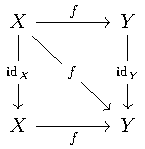
\includegraphics[width=0.8\textwidth]{unit_laws.pdf}
                    \caption{Commutative diagram for Unit Laws}
                    \label{fig: unit_laws}
                \end{minipage} \hspace{0.2\textwidth}
                \begin{minipage}{0.3\textwidth}
                    \centering
                    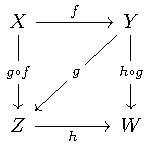
\includegraphics[width=0.8\textwidth]{associativity_law.pdf}
                    \caption{Commutative diagram for Associativity Law}
                    \label{fig: associativity_law}
                \end{minipage}
            \end{figure}

            As examples of commutative diagrams, Figure~\ref{fig: associativity_law} and Figure~\ref{fig: unit_laws} are commutative diagrams for the unit laws and associativity law respectively. 

        
        \subsection{Isomorphism}
        \begin{definition}[Isomorphism]
            Given a category $\mathcal{C}$, a $C$-morphism $f : X \to Y$ is called an \emph{isomorphism} if there exists a $C$-morphism $g : Y \to X$ such that the following diagram commutes:
            \begin{equation}
                \vcenter{\hbox{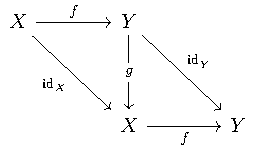
\includegraphics[width=0.3\textwidth]{isomorphism.pdf}}}
                \label{cd: isomorphism}
            \end{equation}
            In other words, $f$ is an isomorphism if there exists a morphism $g$ such that $g \circ f = \textbf{id}_X$ and $f \circ g = \textbf{id}_Y$.

            The morphism $g$ is uniquely determined by $f$ and is called the \emph{inverse} of $f$, denoted as $f^{-1}$.

            Given two objects $X$ and $Y$ in a category $\mathcal{C}$, if there exists an isomorphism from $X$ to $Y$, we say that $X$ and $Y$ are \emph{isomorphic} in $\mathcal{C}$ and write $X \cong Y$.

        \end{definition}

        \subsection{Cartesian closed category}
            \subsubsection{Terminal object}
            \begin{definition}[Terminal object]
                Given a category $\mathcal{C}$, an object $T \in \textbf{obj}(\mathcal{C})$ is called a \emph{terminal object} if for all $X \in \textbf{obj}(\mathcal{C})$, there exists a unique \textbf{C}-morphism $f : X \to T$.
            \end{definition}
            Terminal objects are unique up to isomorphism. In other words, we have the following properties:
            \begin{itemize}
                \item 
                    If $T$ and $T'$ are both terminal objects in $\mathcal{C}$, then there exists a unique isomorphism $f : T \to T'$.
                \item
                    If $T$ is a terminal object in $\mathcal{C}$ and $T \cong T'$, then $T'$ is also a terminal object in $\mathcal{C}$.
            \end{itemize}
            \begin{example}[Terminal object in $\mathcal{Set}$]
                $\mathcal{Set}$ has a terminal object $\{\ast\}$, which is an arbitrary singleton set containing a single element $\ast$.

                For any set $X$, there exists a unique function $f : X \to \{\ast\}$ that maps every element of $X$ to the single element $\ast$ in $\{\ast\}$.
                
                There is a unique isomorphism $f : \{\ast\} \to \{\cdot\}$ for any two singleton sets $\{\ast\}$ and $\{\cdot\}$, which is $f(\ast) = \cdot$.
            \end{example}

            
            \subsubsection{Binary product}
            \begin{definition}[Binary product]
                Given a category $\mathcal{C}$, the \emph{binary product} of two objects $X$ and $Y$ in $\mathcal{C}$ is specified by
                \begin{itemize}
                    \item a $\mathcal{C}$-object $X \times Y$;
                    \item two $\mathcal{C}$-morphisms $\pi_1 : X \times Y \to X$ and $\pi_2 : X \times Y \to Y$ called the \emph{projections} of $X \times Y$;
                \end{itemize}
                such that for all $Z \in \textbf{obj}(\mathcal{C})$ and morphisms $f : Z \to X$ and $g : Z \to Y$, there exists a unique morphism $u : Z \to X \times Y$ such that the following diagram commutes in $\mathcal{C}$:
                \begin{equation}
                    \vcenter{\hbox{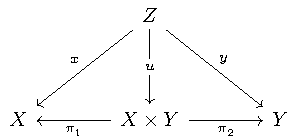
\includegraphics[width=0.4\textwidth]{binary_product.pdf}}}
                    \label{cd: binary_product}
                \end{equation}
                The unique morphism $u$ is written as $\ang{ f, g } : Z \to X \times Y$ where $f = \pi_1 \circ u$ and $g = \pi_2 \circ u$.
            \end{definition}
            It can be shown that the binary product is unique up to (unique) isomorphism.

            \begin{example}[Binary product in $\mathcal{Set}$]
                The binary product of two sets $X$ and $Y$ in $\mathcal{Set}$ is the Cartesian product $X \times Y = \{(x,y) \mid x \in X \land y \in Y\}$, where $(x,y)$ are ordered pairs.

                We have the following projections:
                \begin{itemize}
                    \item 
                        $\pi_1 : X \times Y \to X$ is defined as $\pi_1(x,y) = x$ for all $(x,y) \in X \times Y$;
                    \item
                        $\pi_2 : X \times Y \to Y$ is defined as $\pi_2(x,y) = y$ for all $(x,y) \in X \times Y$.
                \end{itemize}

            
                For any set $Z$, for any functions $f : Z \to X$ and $g : Z \to Y$, the unique morphism $u : Z \to X \times Y$ is defined as:
                \[u(z) = (f(z), g(z)) \text{ for all $z \in Z$.}\]
            \end{example}



            \subsubsection{Exponential}
            \begin{definition}[Exponential]
                Given a category $\mathcal{C}$ with binary products, the \emph{exponential} of two objects $X$ and $Y$ in $\mathcal{C}$ is specified by
                \begin{itemize}
                    \item a $\mathcal{C}$-object $X \Rightarrow Y$;
                    \item a $\mathcal{C}$-morphism $\textbf{app} : (X \Rightarrow Y) \times X \to Y$ called the \emph{application} of $X \Rightarrow Y$;
                \end{itemize}
                such that for all $Z \in \textbf{obj}(\mathcal{C})$ and morphisms $f : Z \times X \to Y$, there exists a unique morphism $u : Z \to X \Rightarrow Y$ such that the following diagram commutes in $\mathcal{C}$:
                \begin{equation}
                    \vcenter{\hbox{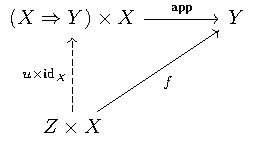
\includegraphics[width=0.4\textwidth]{exponential.pdf}}}
                    \label{cd: exponential}
                \end{equation}
                We write $\textbf{cur} f$ for the unique morphism $u$ such that $f = \textbf{app} \circ (\textbf{cur} f \times \textbf{id}_X)$, 
                where $\textbf{cur} f$ is called the \emph{currying} of $f$.
            \end{definition}
            It can be shown that the exponential is unique up to (unique) isomorphism.

            \begin{example}[Exponential in $\mathcal{Set}$]
                The exponential of two sets $X$ and $Y$ in $\mathcal{Set}$ is the set of all functions from $X$ to $Y$.

                Function application gives the morphism $\textbf{app} : (X \Rightarrow Y) \times X \to Y$ as $\textbf{app}(f,x) = f(x)$ for all $f \in X \Rightarrow Y$ and $x \in X$.

                The currying operation transform a function $f : Z \times X \to Y$ into a function $\textbf{cur} f : Z \to (X \Rightarrow Y)$, which is defined as $\textbf{cur} f(z) = \lambda x.f(z,x)$ for all $z \in Z$ and $x \in X$.

                
            \end{example}

        \begin{definition}[Cartesian closed category]
            A category $\mathcal{C}$ is called a \emph{Cartesian closed category} (CCC) if it has a terminal object, binary products and exponentials of any two objects.
        \end{definition}

        
        \subsection{Functor}
        \begin{definition}[Functor]
            Given two categories $\mathcal{C}$ and $\mathcal{D}$, a \emph{functor} $F: \mathcal{C} \to \mathcal{D}$ is specified by
            \begin{itemize}
                \item 
                    a function 
                    \[\begin{aligned}
                        \textbf{obj}(\mathcal{C}) &\to \textbf{obj}(\mathcal{D}) \\
                        X &\mapsto F(X)
                    \end{aligned}\]

                \item 
                    for each $X, Y \in \textbf{obj}(\mathcal{C})$, a function 
                    \[\begin{aligned}
                        \mathcal{C}{(X,Y)} &\to \mathcal{D}{(F(X),F(Y))} \\
                        f &\mapsto F(f)
                    \end{aligned}\]
            \end{itemize}
            satisfying the following properties:
            \begin{itemize}
                \item 
                    For all $X, Y \in \textbf{obj}(\mathcal{C})$ and $f \in \mathcal{C}{(X,Y)}$, we have: $ F(\textbf{id}_X) = \textbf{id}_{F(X)}$
                \item
                    For all $X, Y, Z \in \textbf{obj}(\mathcal{C})$ and $f \in \mathcal{C}{(X,Y)}$, $g \in \mathcal{C}{(Y,Z)}$, we have: $F(g \circ f) = F(g) \circ F(f)$
            \end{itemize}
        \end{definition}

        
        \subsection{Natural transformation}
        \begin{definition}[Natural transformation]

            Given two categories $\mathcal{C}$ and $\mathcal{D}$, and two functors $F,G: \mathcal{C} \to \mathcal{D}$, a \emph{natural transformation} $\theta : F \to G$ is a family of morphisms $\theta_X \in \mathcal{D}{(F(X),G(X))}$ for each $X \in \textbf{obj}(\mathcal{C})$ such that for all $X, Y \in \textbf{obj}(\mathcal{C})$ and $f \in \mathcal{C}{(X,Y)}$, the following diagram 
            \begin{equation}
                \vcenter{\hbox{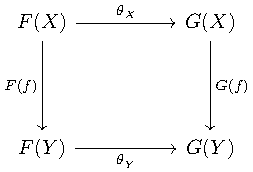
\includegraphics[width=0.3\textwidth]{natural_transformation.pdf}}}
                \label{cd: natural_transformation}
            \end{equation}
            
            commutes in $\mathcal{D}$, i.e. $G(f) \circ \theta_X = \theta_Y \circ F(f)$

        \end{definition}

        
        \subsection{Functor category}
        \begin{definition}[Functor category]
            Given two categories $\mathcal{C}$ and $\mathcal{D}$, the \emph{functor category} $\mathcal{D}^{\mathcal{C}}$ is the category satisfying the following:
            \begin{itemize}
                \item 
                    The objects of $\mathcal{D}^{\mathcal{C}}$ are all functors $\mathcal{C} \to \mathcal{D}$;
                \item 
                    Given two functors $F,G: \mathcal{C} \to \mathcal{D}$, the morphisms from $F$ to $G$ in $\mathcal{D}^{\mathcal{C}}$ are all natural transformations $\theta : F \to G$;
                \item
                    Composition and identity morphisms in $\mathcal{D}^{\mathcal{C}}$ are defined as follows:
                    \begin{itemize}
                        \item 
                            The identity morphism $\textbf{id}_F$ on $F$ is defined as $\theta_X = \textbf{id}_{F(X)}$ for all $X \in \textbf{obj}(\mathcal{C})$;
                        \item
                            The composition of two natural transformations $\theta : F \to G$ and $\phi : G \to H$ is defined as $(\phi \circ \theta)_X = \phi_X \circ \theta_X$ for all $X \in \textbf{obj}(\mathcal{C})$.
                    \end{itemize}
            \end{itemize}
        \end{definition}

        \subsection{Presheaf category}
        \begin{definition}[Presheaf]
            Given a category $\mathcal{C}$, a \emph{presheaf} on $\mathcal{C}$ is a functor $F: \mathcal{C}^{\textbf{op}} \to \mathcal{Set}$.
            A presheaf is a contravariant functor, which means that it reverses the direction of morphisms.
            In other words, a presheaf is a functor that takes objects in $\mathcal{C}$ and assigns them sets, and takes morphisms in $\mathcal{C}$ and assigns them functions between the corresponding sets.
            The presheaf $F$ is defined as follows:
            \begin{itemize}
                \item 
                    For each $X \in \textbf{obj}(\mathcal{C})$, $F(X)$ is a set;
                \item
                    For each $X, Y \in \textbf{obj}(\mathcal{C})$ and $f \in \mathcal{C}{(X,Y)}$, $F(f)$ is a function $F(Y) \to F(X)$.
            \end{itemize}
        \end{definition}

        \begin{definition}[Presheaf category]
            Given a category $\mathcal{C}$, the \emph{presheaf category} $\hat{\mathcal{C}}$ is the functor category $\mathcal{Set}^{\mathcal{C}^{\textbf{op}}}$, which explicitly contains the following:
            \begin{itemize}
                \item 
                    The objects of $\hat{\mathcal{C}}$ are all presheaves on $\mathcal{C}$;
                \item
                    Given two presheaves $F,G: \mathcal{C}^{\textbf{op}} \to \mathcal{Set}$, the morphisms from $F$ to $G$ in $\hat{\mathcal{C}}$ are all natural transformations $\theta : F \to G$.
            \end{itemize}
        \end{definition}



        \subsection{Yoneda lemma}
        \begin{definition}[Yoneda functor]
            Given a category $\mathcal{C}$, the \emph{Yoneda functor} $\yo: \mathcal{C} \to \hat{\mathcal{C}}$ is defined as follows:
            \begin{itemize}
                \item 
                    For each $X \in \textbf{obj}(\mathcal{C})$, $\yo(X)$ is the functor $\mathcal{C}^{\textbf{op}} \to \mathcal{Set}$ defined as:
                    \begin{equation} \label{eq: yoneda_element}
                        \yo(X)(Y) = \mathcal{C}{(Y,X)}
                    \end{equation}
                    For all $Y \in \textbf{obj}(\mathcal{C})$;
                \item
                    For each $X, Y \in \textbf{obj}(\mathcal{C})$ and $f \in \mathcal{C}{(X,Y)}$, $\yo(f)$ is the morphism $\yo(X) \to \yo(Y)$ defined a natural transformation whose component at any given $Z \in \mathcal{C}^{\textbf{op}}$ is given by:
                    \begin{equation} \label{eq: yoneda_morphism}
                        \begin{aligned}
                            (\yo(f))_Z : \mathcal{C}{(Z,Y)} &\to \mathcal{C}{(Z,X)} \\
                            g &\mapsto g \circ f
                        \end{aligned}
                    \end{equation}
                    for all $Z \in \textbf{obj}(\mathcal{C})$.
                \end{itemize}

        \end{definition}

        \begin{theorem}[Yoneda lemma]
            For each small\footnote{Here the smallness condition avoids foundational issues analogous to Russell's paradox. While we omit the formal definition of size due to the space limit here, all constructions in this work preserve smallness.} category $\mathcal{C}$, the \emph{Yoneda lemma} states that for each object $X \in \textbf{obj}(\mathcal{C})$ and each presheaf $F \in \hat{\mathcal{C}}$, there exists a natural isomorphism
            \begin{equation} \label{eq: yoneda_lemma}
                {\hat{\mathcal{C}}}(\yo(X), F) \cong F(X)
            \end{equation}
        \end{theorem}



        \subsection{Cartesian closed structure in presheaf categories} \label{sec: ccc_presheaf}
        \begin{prf}[Cartesian closed structure in presheaf categories]
            Given a small\footnote{See footnote 1.} category $\mathcal{C}$, the presheaf category $\hat{\mathcal{C}}$ is a Cartesian closed category.
            \begin{itemize}
                \item 
                    The terminal object in $\hat{\mathcal{C}}$ is the constant functor $\mathbf{1} : \mathcal{C}^{\textbf{op}} \to \mathcal{Set}$, given by 
                    \begin{equation}
                        \begin{cases}
                            \mathbf{1}(X) = \{\ast\} & \text{for all } X \in \textbf{obj}(\mathcal{C}) \\
                            \mathbf{1}(f) = \textbf{id}_{\{\ast\}} & \text{for all } f \in \mathcal{C}{(X,Y)}
                        \end{cases}
                    \end{equation}

                \item
                    The binary product in $\hat{\mathcal{C}}$ is given by the product of functors, which is defined as follows:
                    \begin{equation}
                        \begin{aligned}
                            (F \times G)(X) &= F(X) \times G(X) \\
                            (F \times G)(f) &= F(f) \times G(f)
                        \end{aligned}
                    \end{equation}

                \item
                    The exponential in $\hat{\mathcal{C}}$ is derived from the Yoneda lemma,
                    \begin{equation}
                        \begin{aligned}
                            G^{F}(X) &= \hat{\mathcal{C}}(\yo(X) \times F, G) \\
                            G^{F}(f)(\theta) &= \theta \circ (\yo(f) \times \textbf{id}_F) \quad \text{for all } \theta \in \hat{\mathcal{C}}(\yo(Y) \times F, G)
                        \end{aligned}
                    \end{equation}
            \end{itemize}
        \end{prf}
        


    \section{Agda}
        \subsection{Basic data types and pattern matching}
        Here is a simple example selected from PLFA~\autocite{plfa} to illustrate the basic data types and pattern matching in Agda. The example is a definition of natural numbers and a plus function.

        \[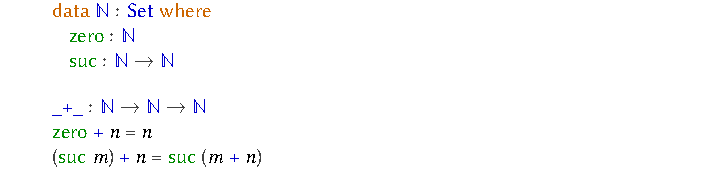
\includegraphics[scale=1.2]{natural_plus.pdf}\]

        In Agda we use the $\og{\mathsf{data}}$ keyword to define a type. Every type has a type, and we use $\mb{\mathsf{Set}}$ to denote the type of all small types. To define a type, we specify its type and its constructors. To define a function, we specify its type and pattern match the input according to the constructors of the type.

        \subsection{Dependent Types}
        A dependent type is a type that depends on a value. In terms of type judgement, simple types are in form of
        \[ x_1 : T_1, x_2 : T_2, \dots, x_n : T_n \vdash t(x_1, \dots, x_n) : T \]
        In contrast, dependent types are in form of
        \[ x_1 : T_1, x_2 : T_2, \dots, x_n : T_n \vdash t(x_1, \dots, x_n) : T(x_1, \dots, x_n) \]
        or more generally
        \[ x_1 : T_1, x_2 : T_2(x_1), \dots, x_n : T_n(x_1, \dots, x_{n-1}) \vdash t(x_1, \dots, x_n) : T(x_1, \dots, x_n) \]

        A classical example of dependent types in Agda is the type of vectors, which are lists with a length. 

        \[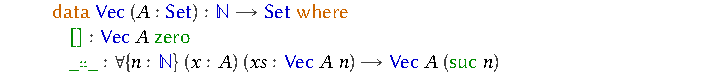
\includegraphics[scale=1.2]{vector.pdf}\]

        Here we define a data type $\mb{\mathsf{Vec}}$ for vectors. The type of vectors is dependent on the length of the vector. With dependent types, we can encode properties directly into types.

        \subsection{Curry-Howard-Lambek correspondence} \label{subsec: curry-howard-lambek}
        Curry-Howard correspondence~\autocite{curry-howard} establishes an isomorphism between logic and type theory, where propositions correspond to types and proofs correspond to terms. This correspondence forms the foundation of functional programming languages that can be used to implement proofs. Building upon this, Joachim Lambek showed that cartesian closed categories provide a natural semantic setting for the simply typed lambda calculus (STLC)~\autocite{lambek}. The Curry-Howard-Lambek correspondence can be summarised as follows:
        \begin{table}[H]
            \centering
            \begin{tabular}{|c|c|c|}
                \hline
                \textbf{Logic} & \textbf{Type theory} & \textbf{Category theory} \\
                \hhline{|=|=|=|}
                Proposition & Type & Object \\
                \hline
                Proof & Term & Morphism \\
                \hline
                Falsity & Empty type & Initial object \\
                \hline
                Truth & Unit type & Terminal object \\
                \hline
                Implication & Function type & Exponential \\
                \hline
                Conjunction & Product type & Product \\
                \hline
                Disjunction & Sum type & Coproduct \\
                % Universal quantification & Dependent product type &  \\
                % Existential quantification & Dependent sum type &  \\
                \hline
            \end{tabular}
            \caption{Curry-Howard-Lambek correspondence}
            \label{tab: curry-howard-lambek}
        \end{table}

        \subsection{Equality, congruence and substitution}\label{subsec: equality}
        Equality here refers to the propositional equality. In Agda it is defined as
        \[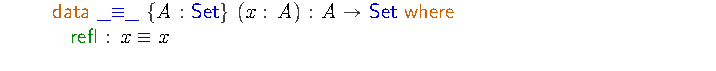
\includegraphics[scale=1.2]{equality.pdf}\]
        With equality as a type, whenever we want to prove that two terms are equal, we need to provide a witness of the equality. For example if we want to prove $x \equiv y$, we write out a term of type $\mb{\mathsf{x = y}}$, and then give its definition, which constructs a proof of the equality. A simple proof that directly uses the definition of equality is as follows:
        \[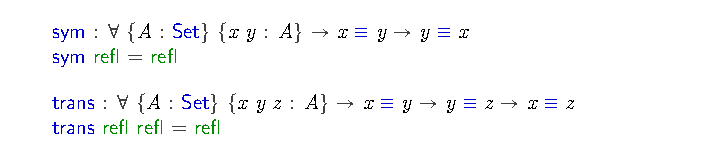
\includegraphics[scale=1.2]{sym_trans.pdf}\]
        Here we are able to prove the symmetry and transitivity of equality by using the definition of equality. Those two properties are very useful for later proofs. 

        We can also have more complex proof with congruence and substitution, which can also be directly derived from the definition of equality as follows:
        \[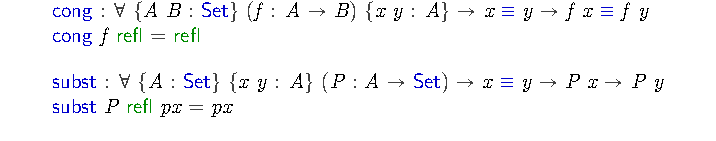
\includegraphics[scale=1.2]{cong_subst.pdf}\]
        Congruence is a property of equality that states that if two terms are equal, then they can be substituted for each other in any context. Substitution is a property where we can get a new proof by replacing a term in a proof with another term that is equal to it. 

        Here is a simple example of how congruence can be used in a proof:
        \[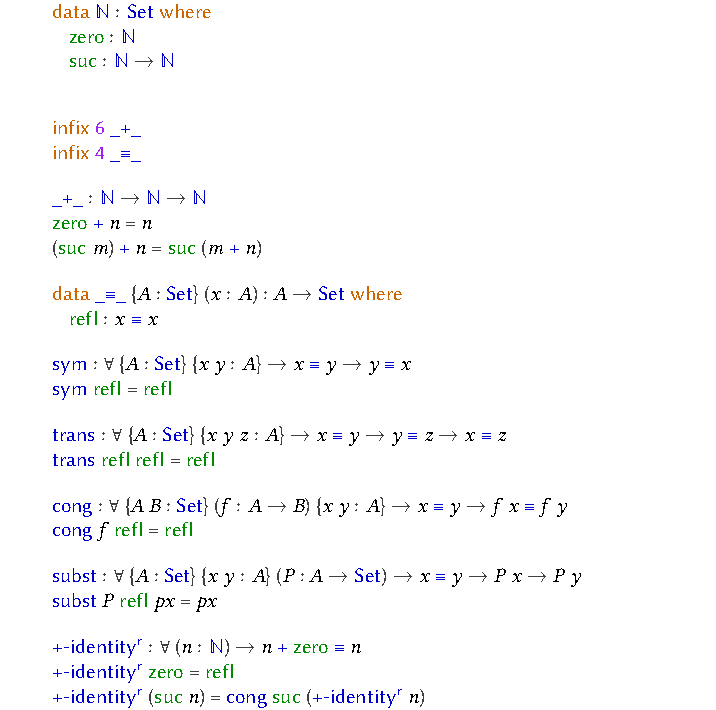
\includegraphics[scale=1.2]{cong_example.pdf}\]

        In this example, we want to prove that $\gn{\mathsf{zero}}$ is the right identity of the plus function. We do an inductive proof by pattern matching on the first argument of the plus function. 
        
        In the base case, we have $\gn{\mathsf{zero}} \mb{{}+{}} \gn{\mathsf{zero}} \equiv \gn{\mathsf{zero}}$, which is trivially true by the definition of the plus function (zero is defined to be the left identity of the plus function). 
        
        In the inductive case, we need to show $\gn{\mathsf{suc}}\ n \mb{{}+{}} \gn{\mathsf{zero}} \equiv \gn{\mathsf{suc}}\ n$. We can use the definition of the plus function to rewrite the left-hand side as $\gn{\mathsf{suc}}\ (n \mb{{}+{}} \gn{\mathsf{zero}})$. By the inductive hypothesis, we know that $n \mb{{}+{}} \gn{\mathsf{zero}} \equiv n$, so we can substitute $n$ for $n \mb{{}+{}} \gn{\mathsf{zero}}$ in the right-hand side by congruence, and we are done.

        % \subsection{With and Rewrite}

        \subsection{Standard library} \label{subsec: stdlib}
        The Agda standard library~\autocite{agda_std} is a collection of modules that provide a wide range of useful functions and types. It includes modules for basic data types, such as natural numbers, lists, and vectors. In my implementation, standard library is used as a reference for defining a customised library, which is specified in~\secref{sec: lib}.

        \subsubsection{Builtin pragma} \label{subsubsec: builtin_pragma}
        With standard library, we can use actual numbers $1, 2, 3, \dots$ instead of calling the constructor $\gn{\mathsf{suc}}$ multiple times. This is a convenient feature for testing. Self-defined functions can be used with the builtin numbers with a \og{\textsf{BUILTIN}} pragma. This allows me to use a convenient syntax of numbers for self-defined functions.
        \[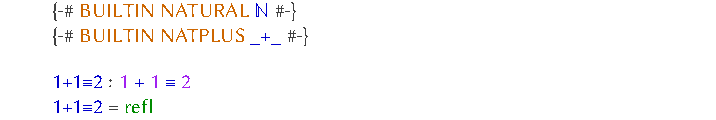
\includegraphics[scale=1.2]{natural_pragma.pdf}\]
        Note that in agda we can use unicode characters for terms, which makes the code more readable. For example, here we simply name the term \mb{1+1$\equiv$2}.

        
        \subsection{Interactive programming with holes} \label{subsec: holes}
        A feature of Agda is interactive programming with holes. By leaving holes in place of undefined terms, we can write programs that are incomplete but still type-check, and Agda's type checker will guide completion of the program: the context window displays inferred types of the holes, available variables and candidate terms with their types. Holes also supports case split and refinement, which means we can fill in a hole partially and split it into smaller holes. 

        In my implementation, I used holes to write the terms in the compiler. The complex terms are incrementally filled and verified by refining partial implementations, reducing post-hoc debugging and ensuring robustness.


    \section{Requirement Analysis}
    To complete the compiler in Agda we need to implement the following components:
    \begin{itemize}
        \item 
            A file \texttt{source.agda} that record the syntax of the source language, which include basic instructions in STLC.

        \item
            A file \texttt{target.agda} that record the syntax of the target language.

        \item
            A file \texttt{compiler.agda} that uses \texttt{source.agda} and \texttt{target.agda} as modules, and write functions whose input is a term in the source language and output is a term in the target language.
        \item 
            A file \texttt{test.agda} that contains test cases for the compiler. The test cases are written in the source language, and the expected output is written in the target language. 
    \end{itemize}
    The success criteria of the project is that all of the above files are implemented and type checked, which ensures that all the terms are well typed and the compilation is as expected.

\chapter{Implementation} \label{chap: implementation}
    \minitoc
    This chapter details the implementation of the compiler in Agda. Starting with a brief overview of the tools used, it then describes the directory structure and file dependencies. Then it discusses the specification of the source language, and the target language, which lead us to the problem of implementing a rigorous natural number subtraction and two different approaches. We will further see the difference between the two approaches and how they affect the implementation of the customised library and the implementation of the compiler. 
    

    \section{Tools used}
    The project is implemented in Agda 2.7.0.1, which is the latest stable version at the time of writing.

    Completing the project is an iterative process. I used Git~\autocite{git} for version control, and work had been synchronised with a GitHub~\autocite{github} repository for backup.

    For the development environment, I tried both Emacs~\autocite{emacs} and Visual Studio Code~\autocite{vscode} with an agda-mode extension~\autocite{agda_mode} on Windows Subsystem for Linux with Ubuntu~\autocite{wsl_ubuntu} 22.04 LTS. I am more familiar with the snippet and syntax highlighting features of Visual Studio Code, so I used it for most of the development. 

    Code from the PLFA tutorial and Agda standard library~\autocite{agda_std} were used as references for implementation of the source language and the customised library. Apart from that, the code is written from scratch.

    \section{Repository Overview}
        \subsection{Directory structure}
        The repository contains two independent implementations of the compiler, organised as follows:
        \dirtree{%
            .1 ..
            .2 fin.
            .3 lib.agda.
            .3 source.agda.
            .3 target.agda.
            .3 compiler.agda.
            .3 test.agda.
            .2 proof.
            .3 lib.agda.
            .3 source.agda.
            .3 target.agda.
            .3 compiler.agda.
            .3 test.agda.
        }

        \subsection{File dependencies and descriptions}
        The dependency graph for each implementation is identical as follows:
        \begin{figure}[H]
            \centering
            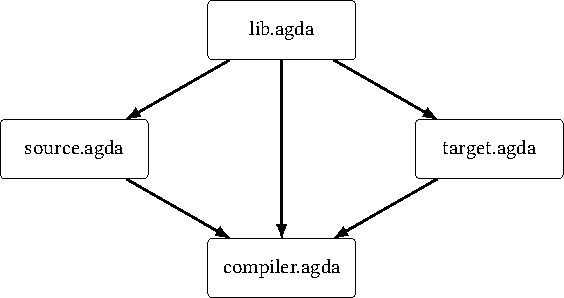
\includegraphics[width=0.6\textwidth]{dependencies.pdf}
            \caption{Dependency graph for the compiler}
            \label{fig: dependencies}
        \end{figure}

        \begin{table}[H]
            \centering
            \begin{tabular}{|l|l|l|}
                \hline
                \textbf{File} & \textbf{Description}\\
                \hhline{|=|=|}
                \texttt{lib.agda} & shared utilities (e.g. natural numbers and operations, equality, etc.) \\
                \hline
                \texttt{source.agda} & source language syntax \\
                \hline
                \texttt{target.agda} & target language (stack machine) instructions \\
                \hline
                \texttt{compiler.agda} & compiler derived from denotational semantics \\
                \hline
                \texttt{test.agda} & test cases for the compiler \\
                \hline
            \end{tabular}
            \caption{File descriptions}
            \label{tab: file_descriptions}
        \end{table}

    \section{Source Language}
    A simply typed lambda calculus (STLC) is a typed lambda calculus with only one type constructor ($\Rightarrow$) \footnote{Normally we use $\to$ to denote the function type, but here we use $\Rightarrow$ to be consistent with the notation in Agda, as $\to$ is a primitive in Agda.} that builds function types. 
    
        \subsection{Types}
        In this dissertation, the source language is an STLC with the following primitive types:
        \begin{itemize}
            \item 
                \textsf{comm}: the commands
            \item 
                \textsf{intexp}: the integer expressions
            \item 
                \textsf{intacc}: the integer acceptors
            \item 
                \textsf{intvar}: the integer variables
        \end{itemize}
        and the set $\Theta$ of types is defined as follows: 
        \[ \Theta := \textsf{comm} \mid \textsf{intexp} \mid \textsf{intacc} \mid \textsf{intvar} \mid \Theta \Rightarrow \Theta \] 
        which corresponds with the following agda implementation:
        \[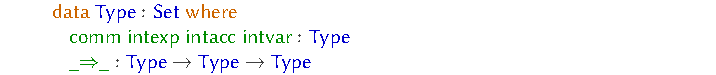
\includegraphics[scale=1.2]{/source/types.pdf}\]

        \subsubsection{Subtypes}
        We use the preorder $A \leq: B$ to denote the subtype relation $A$ is a subtype of $B$, as it has the following properties:
        \begin{itemize}
            \item 
                reflexivity: $A \leq: A$;
            \item 
                transitivity: if $A \leq: B$ and $B \leq: C$, then $A \leq: C$.
        \end{itemize}

        The source language has the following subtype relations:
        \[ \textsf{intvar} \leq: \textsf{intexp} \qquad \textsf{intvar} \leq: \textsf{intacc} \]
        since a variable can be used as an expression (e.g. $\mathsf{x} + 1$) or an acceptor (e.g. $\mathsf{x} := 1$).

        For function types we have the contravariant subtyping:
        \[ A' \leq: A \land B \leq: B' \Rightarrow A \to B \leq: A' \to B' \]
        
        it is defined in Agda as follows:
        \[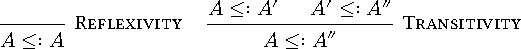
\includegraphics[scale=1.2]{/source/subtype.pdf}\]

        \subsection{Contexts, variables and the lookup judgement}
        We define the context as a finite list of types. When we are looking up a variable, the type of the variable is either the head of the context or in the tail of the context. The definition in Agda is as follows:
        \[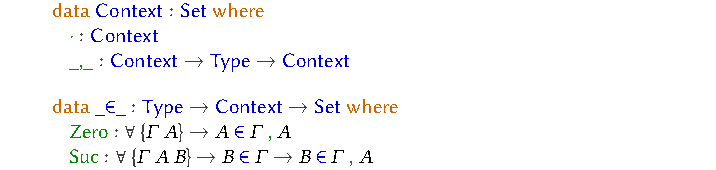
\includegraphics[scale=1.2]{/source/contexts.pdf}\]
        where the $\gn{\mathsf{Zero}}$ case corresponds to the situation where the variable is the head of the context, and the $\gn{\mathsf{Suc}}$ case corresponds to the situation where the variable is in the tail of the context.


        \subsection{Terms and the typing judgement} \label{subsec: terms}
        The terms and the typing judgement are described in the following rules:
        \begin{itemize}
            \item For any variable we have 
                \begin{figure}[H]
                    \centering
                    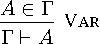
\includegraphics{source_terms_var.pdf}
                    \caption{Variable typing rule}
                    \label{fig: rule_var}
                \end{figure}
            \item For subtyping we have
                \begin{figure}[H]
                    \centering
                    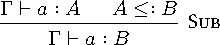
\includegraphics{source_terms_subtype.pdf}
                    \caption{Subtyping rule}
                    \label{fig: rule_subtype}
                \end{figure}
            \item For lambda abstraction we have
                \begin{figure}[H]
                    \centering
                    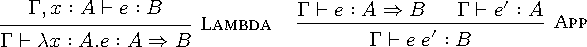
\includegraphics{source_terms_lambda.pdf}
                    \caption{Lambda abstraction typing rules}
                    \label{fig: rule_lambda}
                \end{figure}
            \item For command we have
                \begin{figure}[H]
                    \centering
                    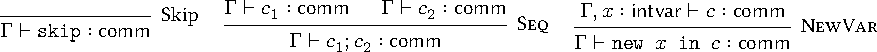
\includegraphics{source_terms_comm.pdf}
                    \caption{Command typing rules}
                    \label{fig: rule_comm}
                \end{figure}
            \item For integer expression we have
                \begin{figure}[H]
                    \centering
                    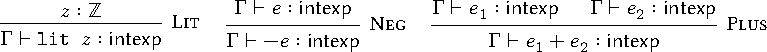
\includegraphics{source_terms_intexp.pdf}
                    \caption{Integer expression typing rules}
                    \label{fig: rule_intexp}
                \end{figure}
        \end{itemize}

        The corresponding Agda implementation is as follows, note that the Agda implementation only does not include the name of the terms, as a term can be specified by how it is constructed (i.e. the name of the typing rules and the corresponding types)
        \[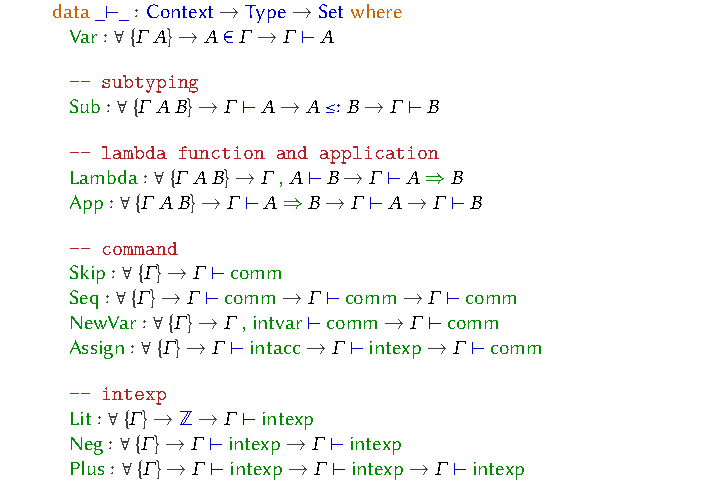
\includegraphics[scale=1.2]{/source/terms.pdf}\]

        Here the definition of the integers $\bZ$ is in the customised library. Please refer to~\secref{sec: lib} for more details.

        \subsection{Operational Semantics}
        The operational semantics of the source language is defined with renaming, substitution and reduction rules. However, since the compiler itself does not require the operational semantics, the implementation is included in Appendix~\ref{app: operational_semantics}. Operational semantics can be used to verify the correctness of the compiler in the future, but it is beyond the scope of this project.


    \section{Target Language}
    The target language is an assembly-style intermediate language for a stack machine. It is defined with four stack-descriptor-indexed families of non-terminals: 
    \begin{itemize}
        \item 
            $\bracket{\textsf{L}_{sd}}$: left-hand sides
        \item 
            $\bracket{\textsf{S}_{sd}}$: simple right-hand sides
        \item
            $\bracket{\textsf{R}_{sd}}$: right-hand sides
        \item
            $\bracket{\textsf{I}_{sd}}$: instruction sequences
    \end{itemize}

    \subsection{Stack descriptor}
    The stack descriptor $sd$ is defined as a pair of natural numbers $\ang{f, d}$, where $f$ is the frame number and $d$ is the displacement. 

    It is defined in Agda as follows:
    \[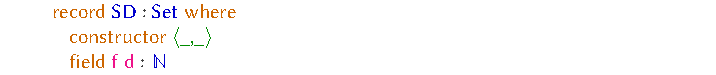
\includegraphics[scale=1.2]{/target/stack_descriptor.pdf}\]
    Here definition of natural numbers is in the customised library. Please refer to~\secref{sec: lib} for more details.

    For a stack descriptor $sd$, we can use \dpink{SD.f} $sd$ to access the frame number and \dpink{SD.d} $sd$ to access the displacement. 

    \subsubsection{Order}
    The stack descriptor is ordered lexicographically with $\leq_s$ as follows:
    \[\ang{f, d} \leq_s \ang{f', d'} \Leftrightarrow f < f' \lor (f = f' \land d \leq d')\]

    It is defined in Agda as follows:
    \[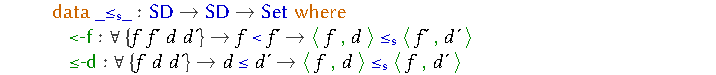
\includegraphics[scale=1.2]{/target/stack_descriptor_order.pdf}\]
    Here definition of the order of natural numbers is in the customised library. Please refer to~\secref{sec: lib} for more details.

    \subsubsection{Addition and subtraction of stack descriptors}
    We define addition and subtraction of stack descriptors as follows:
    \[\ang{f, d} \pm_s n = \ang{f, d \pm n} \text{ for } n \in \mathbb{N}\]
    Addition of stack displacement is defined in Agda as follows:
    \[
\includegraphics[scale=1.2]{/target/stack_descriptor_add.pdf}\]
    For subtraction, we need to make sure that the subtraction is valid, i.e. the subtracted displacement is less than or equal to the displacement of the current stack descriptor. This leads us to the problem of defining the subtraction of natural numbers, which is explained in detail in~\secref{subsec: subtraction}

    \subsubsection{Properties of order and addition}
    We can use reflexivity and transitivity of the order $<$ and $\leq$ to prove that the order of stack descriptors $\leq_s$ is a preorder. The proof is as follows:
    \begin{proof}
        We need to show that $\leq_s$ is reflexive and transitive. 
        \begin{itemize}
            \item 
                Reflexivity: $sd \leq_s sd$ is trivially true since $f = f$ and $d \leq d$.
            \item
                Transitivity: if $\ang{f, d} \leq_s \ang{f', d'}$ and $\ang{f', d'} \leq_s \ang{f'', d''}$, we do the following case split:
                \begin{itemize}
                    \item 
                        If $f < f'$, $f' = f''$ and $d \leq d'$, then $f < f''$; 
                    \item 
                        If $f < f'$ and $f' < f''$, then $f < f''$ by transitivity of $<$;
                    \item
                        If $f = f'$, $d \leq d'$ and $f' < f''$, then $f < f''$;
                    \item
                        If $f = f'$, $d \leq d'$, $f' = f''$ and $d' \leq d''$, then $f = f''$ and $d \leq d''$ by transitivity of $\leq$. \footnote{Note that the properties of $=$ is not required in as in the Agda definition of $\leq_s$, we directly define $f'$ to be $f$ instead of defining a equivalence relation, thus equivalence can be checked directly via type checking.}
                \end{itemize}
        \end{itemize}
    \end{proof}

    The proof is defined in Agda as follows:
    \[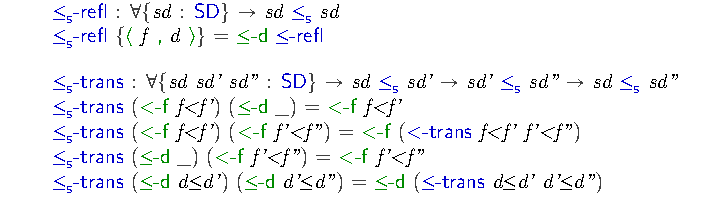
\includegraphics[scale=1.2]{/target/stack_descriptor_order_proof.pdf}\]

    When a natural number is added to a stack descriptor, it is guaranteed that the new stack descriptor is not less than the old stack descriptor. This can be proved directly using the same properties of integer addition. The proof is defined in Agda as follows:
    \[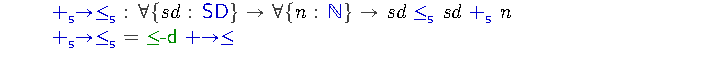
\includegraphics[scale=1.2]{/target/stack_descriptor_add_proof.pdf}\]

    Proof above requires the proof of the properties of natural numbers, which is defined in~\secref{subsec: natural_numbers}.
    

    \subsection{Grammar}
    The grammar of the target language is defined as follows, given the current stack descriptor $sd = \ang{f, d}$, and new stack descriptor $sd'$ and $sd^v$:
    \[\begin{aligned}
        \bracket{\textsf{L}_{sd}} ::={}& sd^v \quad \text{when } sd^v \leq_s sd \\
                        &\mid \texttt{sbrs}  \\
        \bracket{\textsf{S}_{sd}} ::={}& \bracket{\textsf{L}_{sd}} \\
                        &\mid \texttt{lit} \bracket{\text{integer}} \\
        \bracket{\textsf{R}_{sd}} ::={}& \bracket{\textsf{S}_{sd}} \\
                        &\mid \bracket{ \text{unary operator} } \bracket{ \textsf{S}_{sd}}\\
                        &\mid \bracket{\textsf{S}_{sd}} \bracket{\textsf{binary operator}} \bracket{ \textsf{S}_{sd} } \\
        \bracket{\textsf{I}_{sd}} ::={}& \texttt{stop} \\
                        &\left.
                        \begin{aligned}
                        &|{\ } \bracket{\textsf{L}_{sd+\delta}} \gets \bracket{\textsf{R}_{sd}}[\delta] \text{ ; } \bracket{\textsf{I}_{sd+\delta}} \\
                        &|{\ } \texttt{if } \bracket{\textsf{S}_{sd}} \bracket{\text{relational operator}} \bracket{\textsf{S}_{sd}}[\delta] \\
                        & \hphantom{\mid {}} \texttt{ then } \bracket{\textsf{I}_{sd+\delta}} \texttt{ else } \bracket{\textsf{I}_{sd+\delta}} \\
                        &|{\ } \texttt{adjustdisp} [\delta] \text{ ; } \bracket{\textsf{I}_{sd+\delta}} \\
                        \end{aligned}
                        \quad \right\} \text{if } d + \delta \geq 0  \\
                        &{}\mid{} \texttt{popto } sd' \text{ ; } \bracket{\textsf{I}_{sd'}} \quad \text{when } sd' \leq_s sd \\
    \end{aligned}\]

    \subsubsection{Operators}
    The operators are defined as follows:
    \[\begin{aligned}
        \textsf{unary operator} &\in \{\texttt{UNeg}\} \\
        \textsf{binary operator} &\in \{\texttt{BPlus}, \texttt{BMinus}, \texttt{BTimes}\} \\
        \textsf{relational operator} &\in \{\texttt{RLeq}, \texttt{RLt}\}
    \end{aligned}\]

    The operators are defined in Agda as follows:
    \[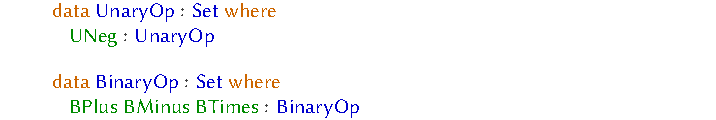
\includegraphics[scale=1.2]{/target/operators.pdf}\]

    \subsubsection{Left-hand sides, simple right-hand sides and right-hand sides}
    The left-hand sides, simple right-hand sides and right-hand sides are straightforward, and they are defined as follows in Agda:
    \[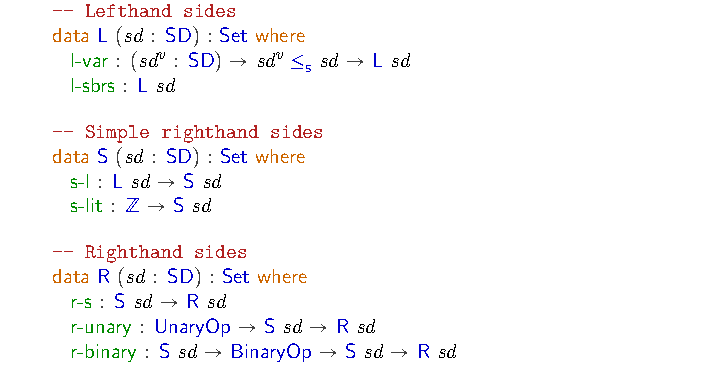
\includegraphics[scale=1.2]{/target/leftrighthand_sides.pdf}\]

    \subsubsection{Instruction sequences}
    In the instruction sequences, $\delta$ as a displacement can be either positive or negative. To make a rigorous definition, we define $\delta$ as a natural number, and treat the positive and negative displacements as two different instructions, using addition and subtraction of stack descriptors respectively. Since the definition of negative displacement involves the rigorous definition of subtraction, we will discuss the subtraction of natural numbers and corresponding implementation in~\secref{subsec: subtraction}. The definition (except for the negative displacement) in Agda is as follows:
    \[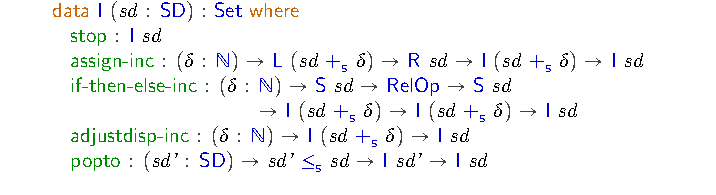
\includegraphics[scale=1.2]{/target/instruction_inc.pdf}\]


    \section{Customised Library} \label{sec: lib}
    The customised library is a collection of types and functions centred around natural numbers, their operations and properties. Instead of using the standard library~\autocite{agda_std}, I implemented a customised library for the following reasons:
    \begin{itemize}
        \item
            \textbf{Specialised Requirements}: The standard library's definitions (e.g. subtraction as monus, `$\dotdiv$') do not align with my project's need for a rigorously defined subtraction operation. This is specified in~\secref{subsec: subtraction}.
        \item
            \textbf{Verification Clarity}: By defining the basic data types and functions from scratch, I can tailor properties (e.g. the property `$n-[n-m] \equiv m$') to my specific requirements, and avoid unnecessary complexity (e.g. `$\leq$' being also defined as a boolean predicate in the standard library). 
        \item
            \textbf{Minimal Dependencies}: Avoiding the standard library reduces external assumptions, making the project self-contained. 
    \end{itemize}

    \subsection{Definition from standard library}
    The following is a list of definitions (or their variants) from the standard library that are used in the customised library:
    \begin{itemize}
        \item 
            Natural numbers, integers and addition.
        \item
            Equality, congruence and substitution.
        \item
            Order of natural numbers, including $\leq$ and $<$.
        \item
            Some properties of order and addition.
    \end{itemize}

    The properties of order and addition contains the following terms summarised in the table below:
    \begin{table}[H]
        \centering
        \begin{tabular}{|l|l|}
            \hline
            \textbf{Agda term} & \textbf{Mathematical meaning} \\
            \hhline{|=|=|}
            $\mb{\mathsf{\mathord{\leq}\text{-}refl}}$ & $\forall n \in \bN, n \leq n$ \\
            \hline
            $\mb{\mathsf{\mathord{\leq}\text{-}trans}}$ & $\forall m, n, p \in \bN, m \leq n \land n \leq p \Rightarrow m \leq p$ \\
            \hline
            $\mb{\mathsf{\mathord{<}\text{-}trans}}$ & $\forall m, n, p \in \bN, m < n \land n < p \Rightarrow m < p$ \\
            \hline
            $\mb{\mathsf{\mathord{<}\mathord{\to}s\mathord{\leq}}}$ & $\forall m, n \in \bN, m < n \Rightarrow \textsf{suc } m \leq n$ \\
            \hline
            $\mb{\mathsf{< \to \leq}}$ & $\forall m, n \in \bN, m < n \Rightarrow m \leq n$ \\
            \hline
            $\mb{\mathsf{\mathord{\leq}\text{-}irrelevance}}$ & $\forall m, n \in \bN$, we consider all proofs of $m \leq n$ to be equal \\
            \hline
            $\mb{\mathsf{\mathord{+}\mathord{\to}\mathord{\leq}}}$ & $\forall m, n \in \bN, m \leq m + n$ \\
            \hline
            $\mb{\mathsf{\mathord{+}\mathord{\to}\mathord{\leq}^r}}$ & $\forall m, n \in \bN, m \leq n + m$ \\
            \hline
        \end{tabular}
        \caption{Properties of order and addition}
        \label{tab: properties}
    \end{table}

    The detailed definitions are included in Appendix~[ref needed].

    % \subsection{Natural numbers, integers and addition} \label{subsec: natural_numbers}
    % The definition of natural numbers, integers and addition is standard, and it is defined as follows:
    % \[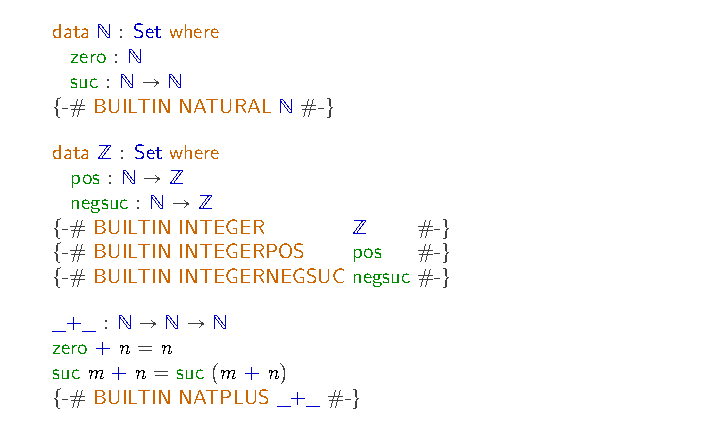
\includegraphics[scale=1.2]{/lib/natural.pdf}\]
    % The use of \og{\textsf{BUILTIN}} is specified in~\secref{subsubsec: builtin_pragma}.

    % \subsection{Equality, congruence and substitution}
    % The definition of equality, congruence and substitution is similar to the one in~\secref{subsec: equality}.\footnote{The definition of equality and related properties in the custom library differ slightly by using an indexed $\mb{\mathsf{Set}}$, which provides a more general formulation. See Appendix [corresponding link].}

    % \subsection{Order of natural numbers} \label{subsec: order}
    % The order of natural numbers we defined include $\leq$ and $<$, we use a simplified definition compared to the one in the standard library as follows:
    % \[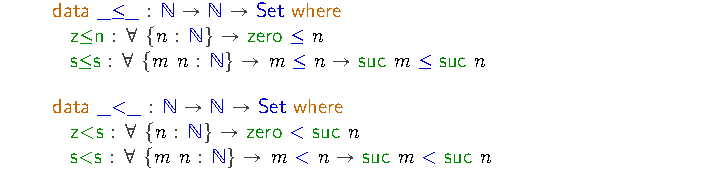
\includegraphics[scale=1.2]{/lib/order.pdf}\]

    % \subsection{Properties of order and addition}
    % \subsubsection{Transitivity and reflexivity}
    % The transitivity and reflexivity of the order $<$ and $\leq$ are defined as follows:
    % \[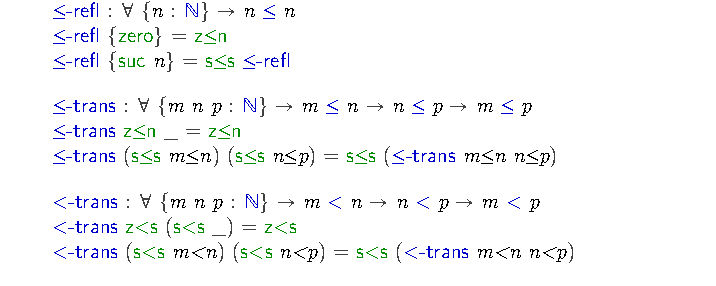
\includegraphics[scale=1.2]{/lib/order_proof.pdf}\]

    % \subsubsection{Implication of order}
    % We know that $\forall m, n \in \bN$, if $m < n$, then we have $m + 1 \leq n$ and $m \leq n$. This is defined in Agda as follows:
    % \[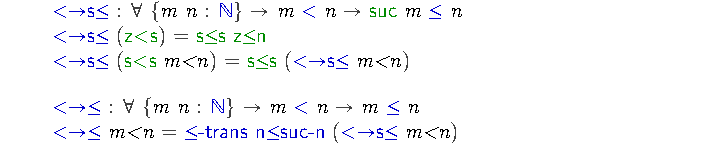
\includegraphics[scale=1.2]{/lib/order_implication.pdf}\]

    \subsubsection{Totality of order}
    It is useful to case split the order of natural numbers, i.e. for any $m, n \in \bN$, we have $m \leq n$ or $n \leq m$. This is defined in Agda by defining either case as an instance of the \mb{\textsf{Total}} type, and then showing that for any $m, n \in \bN$, we can construct a \mb{\textsf{Total}} type by case-split and \og{\textsf{with}}-construct. The proof is as follows:
    \[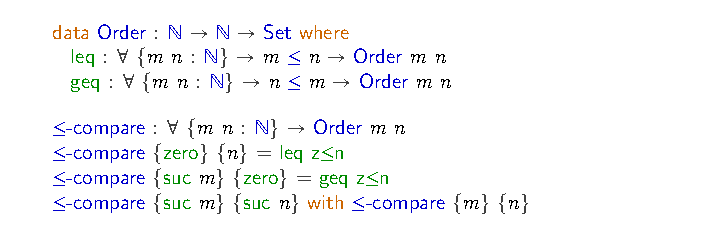
\includegraphics[scale=1.2]{/lib/order_totality.pdf}\]


    % \subsubsection{Other properties}
    % We can show that when a number $n$ is added to a natural number $m$, the result is greater than or equal to $m$. This is defined in Agda as follows:
    % \[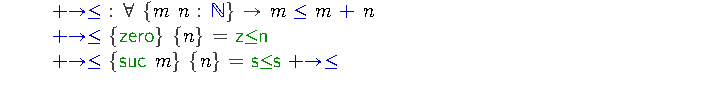
\includegraphics[scale=1.2]{/lib/order_add.pdf}\]


    \subsection{Subtraction} \label{subsec: subtraction}
    In the standard library~\autocite{agda_std}, the subtraction of natural numbers is defined as follows:\footnote{The definition in the standard library directly uses symbol $\mathsf{-}$, but here for clarity we use $\mathsf{\dotdiv}$ instead.}
    \[\includegraphics[scale=1.2]{minus.pdf}\]
    Mathematically we have $ n \dotdiv m = \max(0, n - m)$. This definition is valid and ensures that the result is a natural number. However, there are two problems with this definition for our implementation:
    \begin{itemize}
        \item 
            The definition of subtraction is not rigorous. Input $n$ should be guaranteed not to be less than $m$, and at any point in the program if there is a subtraction where $n < m$, the program should fail to type check instead of making $0$ type check with it.
        \item
            We lose many numerical properties of natural numbers. For example, $n \dotdiv m + m = n$ or $n \dotdiv (n \dotdiv m) = m$ are not guaranteed to hold if we allow $n < m$. Those properties are very useful for the implementation of the compiler.
    \end{itemize}
    We need a more rigorous definition of subtraction that ensures the result is a natural number and preserves the numerical properties. The key is to have a proof that the first argument is greater than or equal to the second argument. There are two approaches to achieve this:

    \subsubsection{Explicit proof-passing approach}
    A straightforward approach is directly include a third argument in the subtraction function, which is a proof that the first argument is greater than or equal to the second argument. The definition in Agda is as follows:
    \[\includegraphics[scale=1.2]{/lib/proof/minus.pdf}\]

    The corresponding implementation for subtraction of stack descriptors carries along the proof as follows:
    \[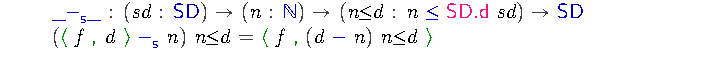
\includegraphics[scale=1.2]{/target/proof/stack_descriptor_minus.pdf}\]

    In the implementation of instruction sequences, we need to carry along the proof as well. The implementation in Agda is as follows:
    \[\includegraphics[scale=1.2]{/target/proof/instruction_dec.pdf}\]

    \subsubsection{\textsf{Fin}-based approach}
    Instead of include the proof directly, we can define the type of the subtrahend as a type that depends on the minuend, where the type encodes the proof. There is a standard library in Agda on finite sets, where a type $\mb{\mathsf{Fin}}$ is defined as a type that depends on a natural number $n$, where $\mb{\mathsf{Fin}}\ n$ can be seen as the set of natural numbers less than $n$. The definition is as follows:
    \[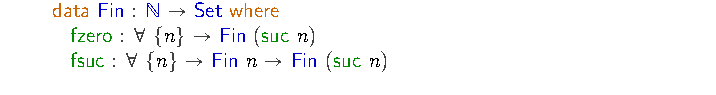
\includegraphics[scale=1.2]{/lib/fin/fin.pdf}\]

    An intuitive explanation of the definition of $\mb{\mathsf{Fin}}$ is as follows:
    \begin{itemize}
        \item Base case: when $n = 0$, there is no element less than $0$, so we do not have any constructor that gives us an element of type $\mb{\mathsf{Fin}}\ 0$. 
        \item Inductive case: 
        \begin{figure}[H]
            \centering
            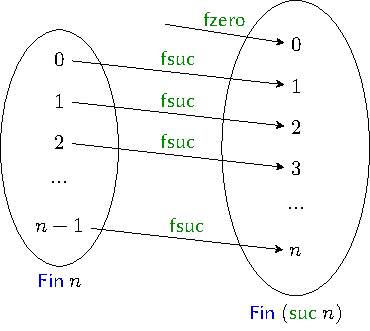
\includegraphics[width=0.35\textwidth]{fin_inductive.pdf}
            \caption{Inductive case of $\mb{\mathsf{Fin}}$}
            \label{fig: fin_inductive}
        \end{figure}
    \end{itemize}

    For subtraction, we only need to change the type of the subtrahend to $\mb{\mathsf{Fin}}\ (\gn{\mathsf{suc}}\ n)$ compared to the implementation of addition. The definition in Agda is as follows:
    \[\includegraphics[scale=1.2]{/lib/fin/minus.pdf}\]

    The corresponding implementation for subtraction of stack descriptors and instruction sequences only requires a change of the type of the subtrahend as follows:
    \[\includegraphics[scale=1.2]{/target/fin/instruction_dec.pdf}\]

    \subsubsection{Comparison of the two approaches}
    The explicit approach carries proofs directly in the type system, which is more transparent but verbose. The $\textsf{Fin}$-based approach intially appears to be more elegant, as it encapsulates bounds check within a refined type. However, this elegance is superficial: constructing a term of type $\mb{\mathsf{Fin}}\ n$ still requires the same underlying proof of boundedness, shifting complexity to auxiliary conversions. 
    
    To prove a property with the $\textsf{Fin}$-based approach, we need the following auxiliary function:
    \[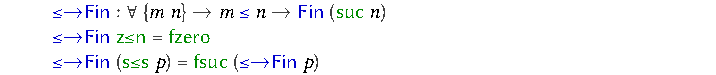
\includegraphics[scale=1.2]{/lib/fin/toFin.pdf}\]

    Here is a comparison of the two approaches representing the property $\mathsf{suc}\ (n - m) \equiv \mathsf{suc}\ n - m$:
    \begin{figure}[H]
        \centering
        \includegraphics[scale=1.2]{/lib/proof/minus-suc.pdf}
        \includegraphics[scale=1.2]{/lib/fin/minus-suc.pdf}
        \caption{Comparison of explicit vs. \textsf{Fin}-based approaches}
        \label{fig: fin_comparison}
    \end{figure}
    The explicit approach's verbosity pays off in readability when representing properties. the type of the term directly mirrors the mathematical statement with an explicit proof. In contrast, the $\textsf{Fin}$-based approach fractures this relationship, and reconstructing the original subtrahend requires tracing the type of the proof. This becomes cumbersome when the proofs are chained inequalities with transitivity, making the code harder to understand.

    Although the project completed both approaches, the following implementation of the compiler uses the explicit proof-passing approach due to its clarity.

    \subsection{More properties of natural numbers}
    The following are some properties of natural numbers that are useful for the implementation of the compiler with corresponding proofs.

    The implementation of the properties of natural numbers in Agda is as follows:
    \begin{figure}[H]
        \centering
        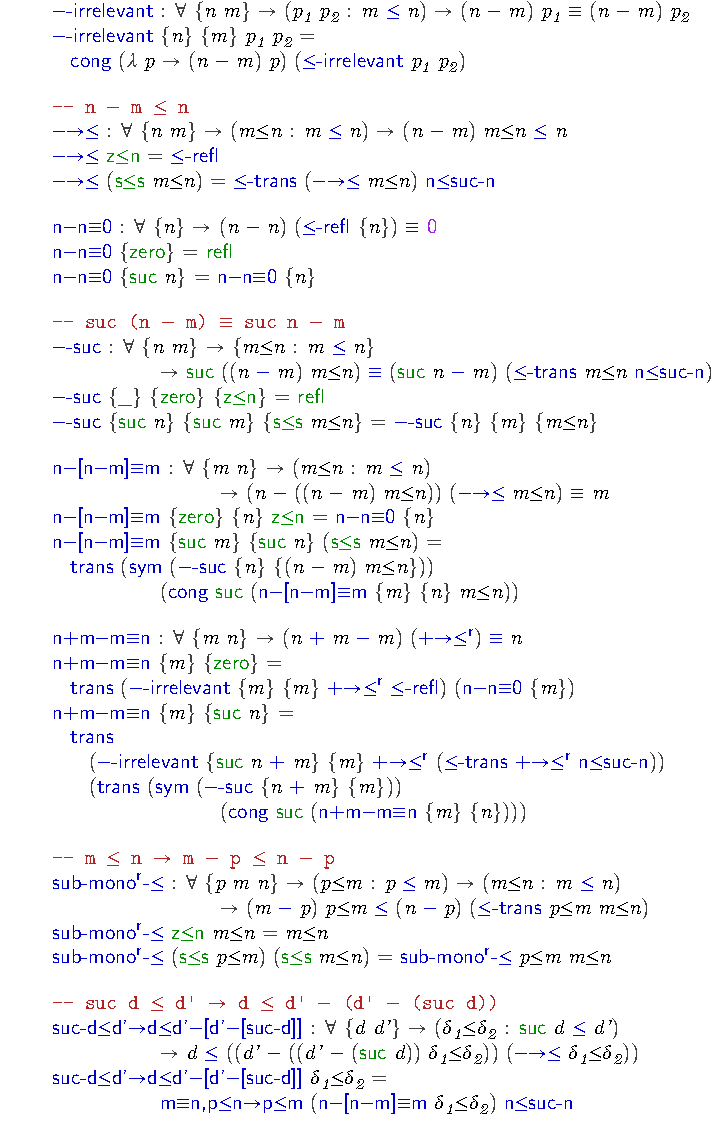
\includegraphics[scale=1.2]{/lib/proof/properties.pdf}
        \caption{Properties of natural numbers related to subtraction}
        \label{fig: properties_subtraction}
    \end{figure}


    

    \section{Compiler}
    \subsection{Presheaf semantics}
    The denotation semantics interprets types as presheaves over a base category $\Upsigma$. 
    \subsubsection{Base category}
    The base category $\Upsigma$ is specified as follows:
    \begin{itemize}
        \item Objects are stack descriptors ($sd = \ang{f, d}$)
        \item Morphisms are stack expansions ($\iota : sd \to sd'$ for $sd \leq_s sd'$) 
    \end{itemize}
    We define $\mathsf{SD}$ as the set of stack descriptors. Then the base category is the category determined by preorder $\underline{\mathsf{SD}} = \{\mathsf{SD}, \leq_s\}$ in Example~\ref{ex: category_preorder}.

    \subsubsection{Semantic category}
    Semantic category $\mathcal{K}$ is the functor category $\text{PDOM}^{\Upsigma^{\textbf{op}}}$, where $\text{PDOM}$ is the category of predomains and continuous functions.
    \begin{itemize}
        \item Objects are presheaves: $P = \Upsigma^{\textbf{op}} \to \text{PDOM}$.
        \item Morphisms are natural transformations: $\eta : P \to Q$ for $P, Q \in \text{PDOM}^{\Upsigma^{\textbf{op}}}$.
    \end{itemize}
    The proof for semantic category is similar to the one in~\secref{sec: ccc_presheaf}, and the full proof is given by Oles in~\autocite{Oles_1, Oles_2}.
    \begin{itemize}
        \item Products are given by pointwise product of presheaves: $P \times Q = \lambda sd.\ P\ sd \times Q\ sd$.
        \item Exponentials $P \Rightarrow_s Q$ are given by the following equation:
            \begin{equation}
                \begin{aligned}
                    P \Rightarrow_s Q &= \lambda sd.\ \mathcal{K}(\yo (sd) \times P, Q) \\
                    &\cong \lambda sd.\{F \mid sd' \in \Upsigma, F : (\yo (sd) \times P)\ sd' \to Q\ sd'\} \\
                    &\cong \lambda sd.\{F \mid sd' \in \Upsigma, F : (\Upsigma(sd, sd') \times P)\ sd' \to Q\ sd'\} \\
                    &\cong \lambda sd.\{F \mid sd' \in \Upsigma, F : sd \leq_s sd' \to P\ sd' \to Q\ sd'\}
                \end{aligned}
                \label{eq: presheaf_exponential}
            \end{equation}
    \end{itemize}
    [need support for each step of the proof]

    The definition of products and exponentials in Agda is as follows:
    \[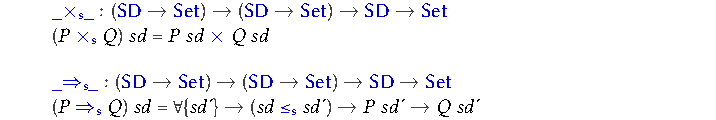
\includegraphics[scale=1.2]{/compiler/product_exponentials.pdf}\]

    We have a functor $\intp{-} : \Theta \to \mathcal{K}$, that interprets the type constructor $\to$ as the exponential functor $\Rightarrow_s$.

    \subsection{Continuations}
    In Reynolds' model, we use $\mathsf{Compl}$ and $\mathsf{Intcompl}$ to represent command and integer continuations. Mathematically we have
    \[\mathsf{Compl } sd : \mathsf{SD} \to O \qquad \mathsf{Intcompl } sd : \bZ \to (\mathsf{SD} \to O)\]
    where $O$ is an unspecified domain of outputs.

    For code generation we define the continuation to be the instruction sequence in the target language:
    \[\mathsf{Compl } sd = \textsf{I}_{sd}\]

    The definition of integer continuation is more complex, it is an exponential object in the presheaf category, which is defined as follows:
    \[\mathsf{Intcompl } = R \Rightarrow_s \mathsf{Compl } \]
    where $R$ is the functor corresponding to the right-hand sides in the target language, $R\ sd = \textsf{R}_{sd}$. Thus we can directly use the definition of $R$ to define the integer continuation as follows:
    \[\includegraphics[scale=1.2]{/compiler/continuations.pdf}\]

    \subsection{Denotational semantics of types and contexts}
    Given the definition of continuations, we can define the denotational semantics of types in Agda as follows:
    \[\includegraphics[scale=1.2]{/compiler/type_interpretation.pdf}\]

    The denotational semantics of contexts is essentially a list expressed by the product of the denotational semantics of the types in the context. The denotational semantics of contexts is defined as follows, where we use $\emptyset$ to denote the denotational semantics of the empty context:
    \[\includegraphics[scale=1.2]{/compiler/context_interpretation.pdf}\]

    \subsection{Morphisms: functorial mapping}
    \[\includegraphics[scale=1.2]{/compiler/fmap_ctx.pdf}\]
    Similarly, this functorial mapping also holds for \textsf{L} and \textsf{S} in the target language. The functorial mapping is defined as follows:
    \[\includegraphics[scale=1.2]{/compiler/fmap_LS.pdf}\]

    \subsection{Denotational semantics of terms}
    The denotational semantics of terms is defined as a morphism from the denotational semantics of contexts to the denotational semantics of types. Similarly, it is a family of continuous functions indexed by the stack descriptor. The denotational semantics of terms has the following type in Agda:
    \[\includegraphics[scale=1.2]{/compiler/term_interpretation_type.pdf}\]

    We need to find out the denotational semantics of the terms corresponding to all rules in the typing judgement mentioned in~\secref{subsec: terms}. 

        \subsubsection{Variables}
        The denotational semantics of variables is defined as follows:
        \[\includegraphics[scale=1.2]{/compiler/term_var.pdf}\]

        \subsubsection{Subtyping}
        The denotational semantics of subtyping is defined as follows:
        \[\includegraphics[scale=1.2]{/compiler/term_subtype.pdf}\]

        \subsubsection{Lambda abstraction}
        The denotational semantics of lambda abstraction is defined as follows:
        \[\includegraphics[scale=1.2]{/compiler/term_lambda.pdf}\]

        \subsubsection{Commands}
        The denotational semantics of commands is defined as follows:
        \[\includegraphics[scale=1.2]{/compiler/term_comm.pdf}\]
        The command \textsf{NewVar} is slightly more complicated, [To complete].

        \subsubsection{Integer expressions}
        The denotational semantics of integer expressions is defined as follows:
        \[\includegraphics[scale=1.2]{/compiler/term_intexp.pdf}\]
        The helper function \textsf{use-temp} is defined as follows:
        \[\includegraphics[scale=1.2]{/compiler/assign_use-temp.pdf}\]

    \subsection{Compilation} \label{subsec: compilation}
    Compilation is a functor from the source language to the target language. To define the compilation functor, we use the denotational semantics of terms and fill in the initial stack descriptor ($\ang{0, 0}$), the empty context (\textsf{unit}), a trivial proof for stack descriptor being not less than itself ($\mathsf{\leq_s-refl}$) and the continuation representing the last instruction (\textsf{stop}):
    \[\includegraphics[scale=1.2]{/compiler/compilation.pdf}\]




\chapter{Evaluation}
    \minitoc
    Chapter~\chapref{chap: implementation} describes the implementation of the source language, the target language and the compiler in Agda. This chapter evaluates the implementation with integration tests and a feature checklist and then discusses the success criteria of the project.
    \section{Tests}
    \subsection{Test cases}
    The correctness of the compiler is evaluated with a set of test cases. Each test is defined as follows
    \begin{figure}[H]
        \centering
        \includegraphics[scale=1.2]{/test/example.pdf}
        \caption{Test 0 as an example of test cases}
        \label{fig: test_case_0}
    \end{figure}
    where definition of the \mb{\textsf{compile-closed}} function is specified in~\secref{subsec: compilation}. The program type checks only if both of the source term and the target term are correctly defined, and the target term is the result of the compilation of the source term. 

    There are special tests to check that some expressions in the source language compiles to the same expression in the target language. Such test is defined as follows:
    \begin{figure}[H]
        \centering
        \includegraphics[scale=1.2]{/test/equivalence.pdf}
        \caption{Test 3' as an example for checking equivalent compiled results}
        \label{fig: test_case_3'}
    \end{figure}

    The full test cases are available in the appendix [insert link]. Here is a summary of the test cases written in a more readable format:
    \begin{enumerate}[label=\textbf{Test \arabic*.}, leftmargin=*]
        \setcounter{enumi}{-1}
        \item $\mathsf{skip}$
        \item $\mathsf{x := 2}$
        \item $\mathsf{x := (\mathnormal{\lambda} a.\ a)\ 4}$
        \item $\mathsf{x := (\mathnormal{\lambda} a.\ (\mathnormal{\lambda} b.\ a+b)\ 2)\ 3}$
        \item[\textbf{Test 3'.}] $\mathsf{x := 3 + 2}$
        \item $\mathsf{x := -3;\ y := (\mathnormal{\lambda} a. x)\ 2}$
        \item $\mathsf{x := 2;\ x := x + 1}$
        \item[\textbf{Test 5'.}] $\mathsf{x := 2;\ skip;\ x := x + 1}$
        \item $\mathsf{x := 2;\ x := -x + 1}$
        \item $\mathsf{x := (\mathnormal{\lambda} a.\ -a+1)\ 2}$
    \end{enumerate}
    where \textbf{Test 3} and \textbf{Test 3'}, \textbf{Test 5} and \textbf{Test 5'} compile to the same target term. 
    
    \textbf{Test 3} and \textbf{Test 3'} are equivalent in terms of compilation because the compilation directly substitutes the value in corresponding lambda terms. 
    
    \textbf{Test 5} and \textbf{Test 5'} are equivalent in terms of compilation because $\mathsf{skip}$ is a no-op in the source language.

    \subsection{Feature checklist}
    Traditional unit tests are not suitable for this project, as many typing judgement rules cannot be tested in isolation. For example, testing subtyping rule (Figure~\ref{fig: rule_subtype}) or any of the integer expression typing rules (Figure~\ref{fig: rule_intexp}) inherently requires embedding them in a well-typed command (\textsc{NewVar} in Figure~\ref{fig: rule_comm}), as the compiler only accepts complete commands. 

    Instead, I employed integration testing with a feature checklist, ensuring comprehensive coverage by validating all typing rules and targeting edge cases.
    \begin{table}[H]
        \centering
        \begin{tabular}{| c | c | c | c |}
            \hline
            \textbf{Feature}  & \textbf{Typing judgement} & \textbf{Specification} & \textbf{Test cases number} \\
            \hhline{|=|=|=|=|}
            Variable & \textsc{Var} & - & 1, 2, 3, 3', 4, 5, 5', 6, 7 \\ \cline{3-4}
            \hline
            \multirow{2}{*}{Subtyping} 
                & \multirow{2}{*}{\textsc{Sub}} 
                    & \textsf{intvar} $\leq:$ \textsf{intacc} & 1, 2, 3, 3', 4, 5, 5', 6, 7  \\ \cline{3-4}
                &   & \textsf{intvar} $\leq:$ \textsf{intexp} & 4, 5, 5', 6 \\
            \hline
            \multirowcell{4}{Lambda\\abstraction} 
                & \multirow{3}{*}{\textsc{Lambda}} 
                    & - & 2, 3, 4, 7 \\ \cline{3-4}
                &   & Multiple variables\hyperlink{note1}{$^{\ast}$} & 3  \\ \cline{3-4}
                &   & Free variables\hyperlink{note1}{$^{\ast}$} & 4 \\ \cline{2-4}
                & \textsc{App} & - & 2, 3, 4, 7  \\
            \hline
            \multirow{7}{*}{Command} 
                & \textsc{Skip} & - & 0, 5' \\ \cline{2-4}
                & \multirow{2}{*}{\textsc{Seq}} 
                    & - & 4, 5, 5', 6 \\ \cline{3-4}
                &   & Multiple sequencing & 5' \\ \cline{2-4}
                & \multirow{2}{*}{\textsc{NewVar}} 
                    & - & 1, 2, 3, 3', 4, 5, 5', 6, 7 \\ \cline{3-4}
                &   & Multiple variables\hyperlink{note1}{$^{\ast}$} & 4 \\ \cline{2-4}
                & \multirow{2}{*}{\textsc{Assign}} 
                    & -  & 1, 2, 3, 3', 4, 5, 5', 6, 7  \\ \cline{3-4}
                &   & Self-referential assignments & 5, 5', 6 \\
            \hline
            \multirowcell{5}{Integer\\expression} 
                & \multirow{2}{*}{\textsc{Lit}}  
                    & Natural number  & 1, 3, 3', 4, 5, 6, 7 \\ \cline{3-4}
                &   & Negative number & 2, 4 \\ \cline{2-4}
                & \textsc{Neg} & - & 5, 5', 6, 7  \\ \cline{2-4}
                & \textsc{Plus} & - & 3, 3', 6, 7  \\ \cline{2-4}
                & -             & Multiple expressions\hyperlink{note2}{$^{\dagger}$} & 6, 7 \\
            \hline
        \end{tabular}

        \caption{Feature checklist}
        \label{tab: feature_checklist}
    \end{table}

    Here are some notes on the feature checklist:

    \hypertarget{note1}{$^{\ast}$} These tests ensure that the translation of context as a whole is correct.

    \hypertarget{note2}{$^{\dagger}$} This type of test is necessary because the target language does not support doing multiple operations in a single simple instructions. This is specified in [Implementation section]. As a result, special tests are required to check that the compiler correctly translates multiple integer operations into a continuation of simple instructions defined in the target language. 

    \vspace{2.5em}

    The feature checklist includes all the typing rules in the source language, including edge cases including multiple variables, free variables and self-referential assignments. Additionally, I account for target-language-specific constraints, ensuring multiple operations are translated into simple instructions with continuation. The tests cover all the cases in the feature checklist, ensuring that the compiler generates expected target code under all circumstances.

    \section{Extensibility}
    This project is inherently extensible, as all of the components are defined as terms and types in Agda. The compiler can be extended to support more features by adding new terms in the form of type judgement rules in the source language, adding any new instructions in the target language if needed, and write corresponding compilation rules.

    \section{Success criteria}
    The project has met the success criteria as follows:
    \begin{itemize}
        \item
            A formalisation of the source language has been given in Agda, which includes the syntax, typing rules and operational semantics. 

        \item
            A formalisation of the target language has been given in Agda, which includes all instructions from the instruction set. Rigorous definitions of the operation of the stack descriptors are given, ensuring correctness and preserving the mathematical properties of the stack descriptors.
        
        \item
            A formalisation of the compiler has been given in Agda, which includes the denotational semantics of the source language and a term for compilation.

        \item 
            Integration tests have been given in Agda, which cover all the case in the feature checklist. The tests ensure that the compiler generates expected target code under all circumstances.
    \end{itemize}

    The following are the extension criteria that are met:
    \begin{itemize}
        \item 
            A customised library have been developed, which includes rigorous definitions of subtraction of natural numbers and corresponding properties. Two approaches to rigorous definition of subtraction has been implemented and compared.
        \item
            Operational semantics of the source language has been defined with renaming, substitution and reduction rules.
        \item
            usetmp [to be completed]

    \end{itemize}

\chapter{Conclusion}
    \minitoc
    \section{Results}
    This project has successfully implemented a compiler from a source language (STLC with store) to a target language (stack machine) in Agda. The compiler is defined as a functor from the source language to the target language, which is directly generated from the denotational semantics of the source language. The compiler validates and refines Reynolds' theory~\autocite{Reynolds}, offers a concrete example of how category-theoretic semantics can generate intermediate code.

    \section{Lessons learned}
    The project has been quite challenging as I have to learn both category theory and Agda from scratch, and apply them to implementation. The implementation process revealed unexpected gaps between Reynolds' theoretical framework and the computational realisation: while his denotational semantics provided core definitions, actualising them in Agda required formalising numbers, their operations, and properties and diagnosing and resolving type mismatches and ambiguities in the original paper~\autocite{Reynolds}. These hurdles highlighted how even meticulously defined theories can be complicated when translated to working systems.


    In terms of planning the project, the project has deviated slightly from the original timetable in the project proposal due to differences
    between the anticipated structure of the project and its actual development process. When I was drafting the proposal, I expected the workflow to be similar to a standard compiler, so I divided the work into components including basic instructions, variable declarations and conditionals, allocating two weeks for each. In hindsight, these components are similar term definitions, while the core of the project can be more accurately divided into three main tasks: defining the source language, defining the target language, and defining the translation between the two. The most time-consuming aspect of each step has been understanding their formal definitions in the paper and addressing the missing details in the Agda implementation.

    Overall, the project has been a valuable learning experience, and I have gained a deeper understanding of both Category Theory and Agda and an exciting glimpse of how the correspondences between logic, type theory and category theory can be used to implement a compiler.


    \section{Future work}
    The project has successfully implemented the compiler, but there are still many areas for improvement and further research:
    \begin{itemize}
        \item 
            The compiler can be extended to support more features, such as subroutines and iterations.
        \item
            The operational semantics of the target language can be defined, which can be used, along with the operational semantics of the source language, to prove the correctness of the compiler.
        \item
            Reynolds pointed out that the requirement of instructions being natural transformation must be relaxed to allow for instruction sequences that differ operationally but are equivalent in terms of denotational semantics~\autocite[Ch. 6]{Reynolds}. Extra research can be done to develop a reasonable equational theory that can be stated directly on the instruction sequences, under which the semantics actually becomes a true functor category model (i.e. naturality holds).
    \end{itemize}

\printbibliography

\appendix

\chapter{Operational Semantics of the source language} \label{app: operational_semantics}
    \minitoc
    The operational semantics of the source language is defined with renaming, substitution and reduction rules. The implementation is as follows:
    \begin{figure}[H]
        \centering
        \includegraphics[scale=1.2]{/source/operational_semantics_1.pdf}
        \caption{Operational semantics of the source language (Part 1)}
        \label{fig: operational_semantics_1}
    \end{figure}
    \begin{figure}[H]
        \centering
        \includegraphics[scale=1.2]{/source/operational_semantics_2.pdf}
        \caption{Operational semantics of the source language (Part 2)}
        \label{fig: operational_semantics_2}
    \end{figure}


\cleardoublepage
\let\cleardoublepage\clearpage
\pagestyle{empty}
\pagenumbering{gobble}
\includepdf[pages=-, fitpaper=true, pagecommand={}]{final_proposal.pdf}
\AtBeginShipoutNext{\AtBeginShipoutDiscard}
\end{document}